\documentclass{article}
\usepackage{graphicx}
\usepackage[margin=1.5cm]{geometry}
\usepackage{amsmath}

\begin{document}

\title{Unit 7 Lab Activity Conservation of Energy}
\author{Prof. Jordan C. Hanson}

\maketitle

\section{Introduction}

Imagine a weight hanging on a spring, subject to two forces: the force of gravity and the spring force (see Fig. \ref{fig:spring}).

\begin{figure}[ht]
\centering
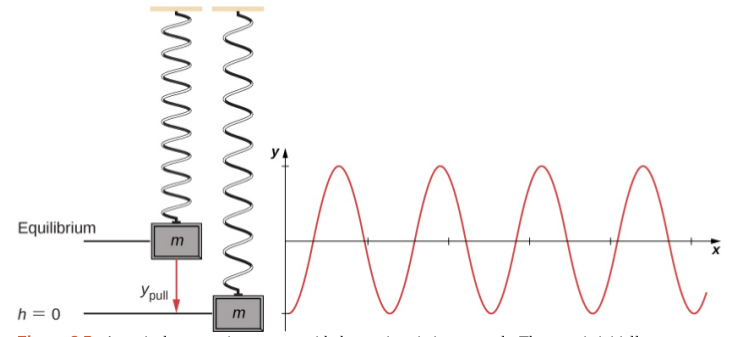
\includegraphics[width=0.5\textwidth,trim=0cm 0.2cm 0cm 0.5cm,clip=true]{figures/osc.png}
\caption{\label{fig:spring} A weight oscillates on a spring.}
\end{figure}

At equilibrium, the spring is exactly the length required to balance gravity with the spring force.  The spring is stretched by an amount $\Delta y$ that depends on the $k$-value.  The $k$-value can be measured by hanging a known weight on the spring and measuring $\Delta y$:

\begin{align}
k(\Delta y) &= mg \\
k &= \frac{mg}{\Delta y}
\end{align}

The net force is

\begin{equation}
F_{\rm net} = ky_{\rm pull} - mg
\end{equation}

Substituting for $k$:

\begin{equation}
F_{\rm net} = \left(\frac{mg}{\Delta y}\right) y_{\rm pull} - mg
\end{equation}

Because $|\Delta y| < |y_{\rm pull}|$, the net force is upwards.  Using Newton's Second Law, we find that

\begin{equation}
a = g\left(\frac{y_{\rm pull}}{\Delta y} - 1\right)
\end{equation}

The acceleration would have the same value but be oriented downward if the spring had been pushed upward by a distance $y_{\rm pull}$ from equilibrium, by symmetry.  In general, the acceleration will always point towards the equilibrium position, and have a value

\begin{equation}
a = g\left(\frac{y}{\Delta y} - 1\right) \label{eq:eq1}
\end{equation}

\section{Conservation of Energy}

Equation \ref{eq:eq1} implies that if the mass is lowered by $y_{\rm pull}$, when it returns to equilibrium, it will have been accelerated to a velocity $v$, and thus have a kinetic energy of $\frac{1}{2}mv^2$, despite having a net force of zero.  The acceleration, however, depends on the position $y$ above the zero-point, and is therefore not constant.  Thus, constant acceleration equations may not be used to predict the velocity.  Energy conservation, however, may be used to predict it.

Let the initial potential and kinetic energy of a system be $U_i$ and $K_i$ respectively.  Let $U_f$ and $K_f$ represent the final potential and kinetic energies.  Conservation of energy states that

\begin{equation}
U_{\rm i} + K_{\rm i} = U_{\rm f} + K_{\rm f} \label{eq:encon}
\end{equation}

Assume that the initial state is when the spring is pulled down by $y_{\rm pull}$, and the final state is equilibrium.  The initial energies are

\begin{align}
U_{\rm i} &= m g (0) + \frac{1}{2}ky_{\rm pull}^2 \\
KE_{\rm i} &= 0
\end{align}

The final energies are

\begin{align}
U_{\rm f} &= m g (y_{\rm pull}) + \frac{1}{2}k(0)^2 \\
KE_{\rm f} &= \frac{1}{2}mv^2
\end{align}

\begin{enumerate}
\item 
Apply energy conservation to show that

\begin{equation}
v = \left( \frac{k}{m} y_{\rm pull}^2 - 2 g y_{\rm pull} \right)^{1/2} \label{eq:pred}
\end{equation}

\vspace{2cm}
\item
Use the LabPro system with motion detector, along with the hanging mass and spring to measure the maximum velocity of the mass.  In a prior lab experiment, we measured the $k$ value.  Insert this value of $k$ into Eq. \ref{eq:pred}, along with $g$ and the value used for $y_{\rm pull}$.  Does the measured velocity agree with the predicted velocity?  Why or why not? \\ \vspace{2cm}
\item
Why does the mass rise to a height of $2y_{\rm pull}$?  Can you justify this based on energy conservation?  Explain in your own words.
\end{enumerate}
\end{document}